\documentclass{article}
\usepackage[margin=2.5cm]{geometry}
\usepackage{enumerate, fancyhdr, graphicx, amsmath}

\def\tetris{Tetris\textsuperscript{\textregistered}}

\title{Old School \tetris{} Meets Machine Learning}
\author{Paul Chesnais (pmc85) and Sam Svenningsen (sjs382)}
\date{\today}

\pagestyle{fancy}
\fancyhead{}
\lhead{pmc85 and sjs382}
\chead{Old School \tetris{} Meets Machine Learning}
\rhead{\today}
\fancyfoot{}
\rfoot{\thepage}
\lfoot{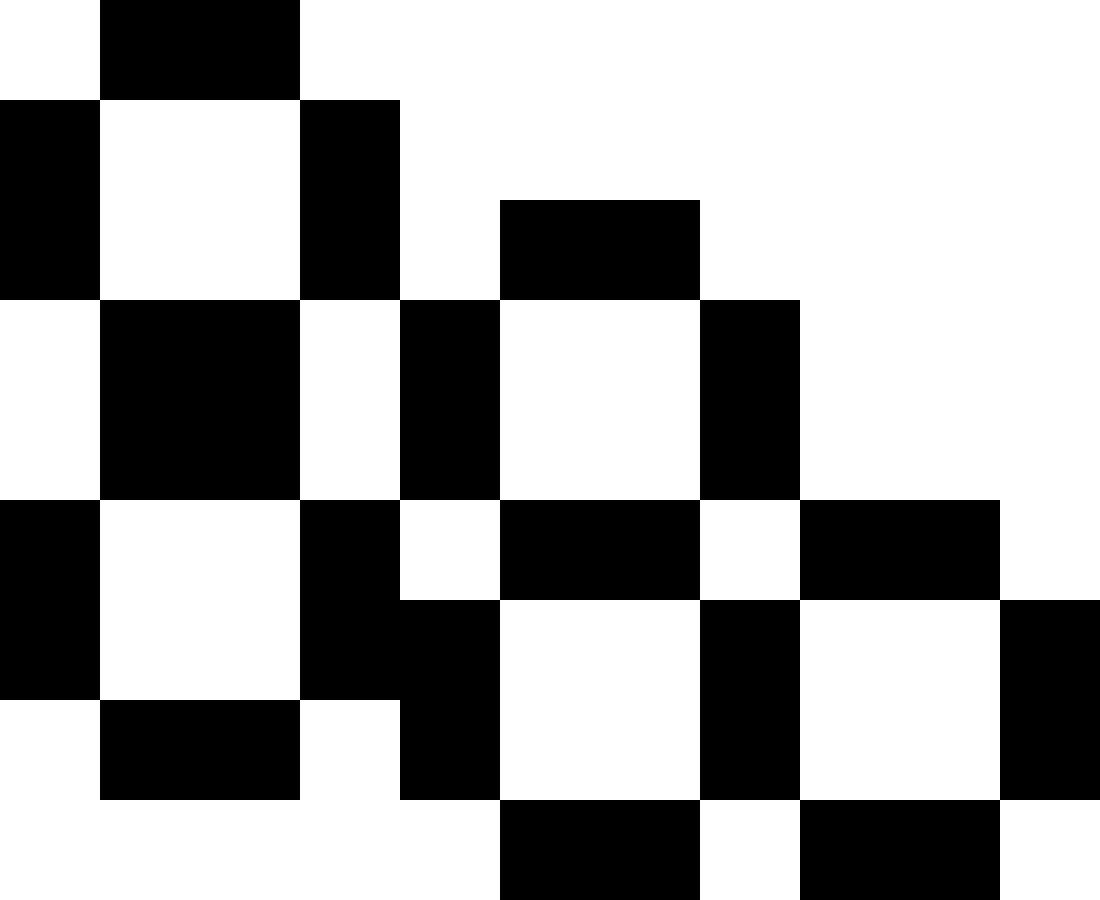
\includegraphics[height=20pt]{Logo}}
\renewcommand{\headrulewidth}{0.5pt}
\renewcommand{\footrulewidth}{0.5pt}

\newcommand{\exo}[1]{\section*{Exercise #1}}
\newcommand{\prob}[1]{\section*{Problem #1}}
\newcommand{\quest}[1]{\section*{Question #1}}
\newcommand{\e}{&=&}
\newcommand{\p}[1]{\times 10^{#1}}

\begin{document}
\maketitle
\thispagestyle{empty}

\section{Description}

\par For our Project in the AI Practicum, we plan on building a \tetris{} bot. Ideally, this bot would play at speeds far greater than normal human speed, and if at all possible, when faced with the original implementation of \tetris{}, would beat the current human world record. We believe that such a task would be quite interesting to attack, and if done well, could in fact teach us a lot about what it is like to play a ``perfect'' \tetris{} game, or what strategies seem to work better than most.



\section{Possible approaches}

\par There are multiple ways to approach solving, or playing, \tetris{}. For shorthand, we will refer to the current state of the game or the ``board'', i.e. all the stacked pieces, as the stack; we will refer to any given instance of having to choose how to use a piece a turn.

\subsection{Informed Search}
An obvious choice would be to, given a particular piece, attempt to place in every rotation and every position, and according to some cost metric, pick the least expensive or most likely to create a good board for the next piece. If we have a lookahead, i.e. we know what piece is coming next, like in most popular \tetris{} games, we can even try all the combinations of each piece and pick which is best. Unfortunately, this method might actually take a while to compute, and may not finish computing until the piece drops and we lose control of it.

\subsection{Ranking}
There is another method in which we look at the game completely differently. Suppose we want to enforce a guarantee that at all times, none of the pieces we have placed have created a hole in the stack. In other words, no hole is created that cannot be filled immediately with the right piece. If this is the case then the only thing we need to look at is the shape of the top layer, let's call it the contour. Suppose we managed to rank every single contour, then all we need to do is pick the position of the falling piece that creates the best ranking contour among the positions that create no hole.

\subsection{Reinforcement Learning}

\section{Plan}

\subsection{Informed Search}
\subsubsection{MINIMAX} We know the current piece and the piece after it, but not the pieces that come after. So it would make sense to try to maximize the next two pieces placement in a way that would minimize the possible damage/maximize the least expected outcome of the next few pieces by using the mimimax approach.

\subsection{Ranking}
Google's PageRank algorithm does something very similar to what we want to achieve with this strategy. We can begin by simplifying contours into a sequence of incremental changes in height going left to right. This should be hashable and therefore very efficient to memoize. We then can compute the rank of all possible contours iteratively, and rank them. With this, we simply throw the algorithm against a sequence of \tetris{} pieces and see how it does.

\subsection{Reinforcement Learning}
\subsubsection{Randomizer} We know the internals of how \tetris{} generates which pieces it is going to use next, so trying to leverage that to learn about what the next possible pieces will be could be useful. For instance, in some approaches, \tetris{} will go out of its way to try to not use a piece that was used in the previous 4 turns, so we can incorporate that into our probability tree.

\section{Timeline}

\par First, we will begin by building some sort of framework against which to test different strategies. We will do this together. Building it involves creating a set of classes representing each of the \tetris{} pieces. Then we need methods which simulate stacking and dropping those pieces. Then we need to implement the random generator that implements which piece comes next. For this, we will do our best to implement something that's as close as possible to the original generator, or at least an official one. Once our methods run relatively efficiently, we might also want to implement a timer that halts the execution of the decision methods if they run too long, to simulate a human running out of time as the piece drops to the bottom of the board.

\par Once the boilerplate is out of the way, we can get to the fun stuff. That is, we can test the two different strategies outlined in this proposal. We will each work on a different strategy, Paul on the Ranking strategy and Sam on the Graph Traversal. This will give us some sort of reference point for our strategies' performance, which be a very valuable asset.

\par At the same time as we are developing our strategies, we will also write a GUI to present our final project but also be able to visualize our progress.

\end{document}